\section{Empirical Results}
\label{sec:results}

\subsection{Forecast degradation under missing history}
Across 48 dataset--mask--rate cells, deterministic error rises as more historical values are removed. Table~\ref{tab:fixed-mask-degradation} gives the representative matrix and Figure~\ref{fig:missingness-degradation} shows the complete rate trends; full tables appear in the supplement.

\begin{table}[t]
\centering
\caption{Deterministic forecast degradation under fixed historical masks. MSE is lower-is-better; relative degradation uses the corresponding clean TimePerceiver forecast as reference.}
\label{tab:fixed-mask-degradation}
\scriptsize
\resizebox{\linewidth}{!}{\begin{tabular}{@{}lrrrr@{}}
\toprule
Dataset & Mask & Rate & MSE & Clean degradation \\
\midrule
ETTh1 & Block & 0.30 & 0.423837 & 13.19\% \\
ETTh1 & Channel & 0.30 & 0.583704 & 55.88\% \\
ETTh1 & Mixed & 0.30 & 0.495055 & 32.20\% \\
ETTh1 & Random & 0.10 & 0.378811 & 1.16\% \\
ETTh1 & Random & 0.30 & 0.425394 & 13.60\% \\
ETTh1 & Random & 0.50 & 0.525856 & 40.43\% \\
Electricity & Block & 0.30 & 0.184630 & 47.28\% \\
Electricity & Channel & 0.30 & 0.391038 & 211.92\% \\
Electricity & Mixed & 0.30 & 0.246785 & 96.86\% \\
Electricity & Random & 0.10 & 0.138429 & 10.42\% \\
Electricity & Random & 0.30 & 0.200572 & 59.99\% \\
Electricity & Random & 0.50 & 0.325732 & 159.83\% \\
Weather & Block & 0.30 & 0.180420 & 25.24\% \\
Weather & Channel & 0.30 & 0.284471 & 97.47\% \\
Weather & Mixed & 0.30 & 0.224939 & 56.14\% \\
Weather & Random & 0.10 & 0.169631 & 17.75\% \\
Weather & Random & 0.30 & 0.240810 & 67.16\% \\
Weather & Random & 0.50 & 0.331313 & 129.99\% \\
\bottomrule
\end{tabular}
}
\end{table}

\begin{figure}[t]
\centering
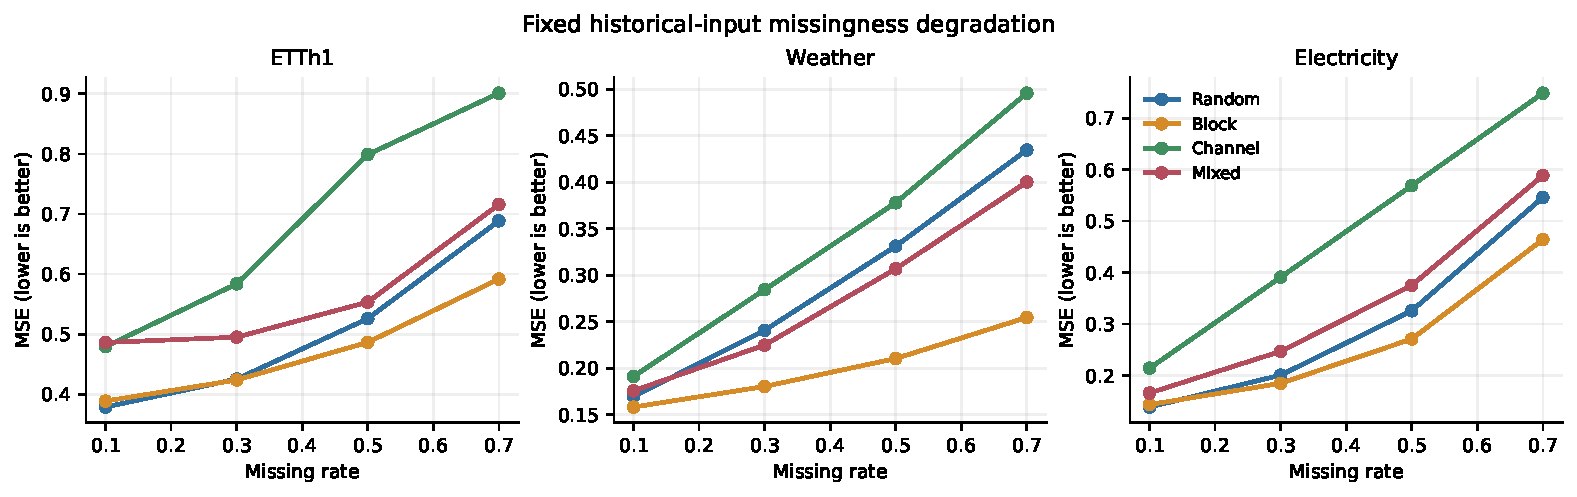
\includegraphics[width=0.96\linewidth]{fig1_missingness_degradation.pdf}
\caption{MSE under fixed historical-mask assets. Line styles and markers distinguish mask types in addition to color, and larger missing rates generally increase forecast error.}
\label{fig:missingness-degradation}
\end{figure}

\subsection{TimePerceiver paired proper-score results}
Across 12 dataset--seed pairs, the \StudentT{} variant improves NLL in 12/12 cases, is CRPS-noninferior in 12/12 cases, and satisfies point noninferiority in 12/12 cases. These are four probability-head seeds on a fixed backbone checkpoint for each dataset. Table~\ref{tab:timeperceiver-multiseed} reports dataset means and variability; Figure~\ref{fig:timeperceiver-nll} retains every paired NLL delta.

\begin{table}[t]
\centering
\caption{TimePerceiver results across four probability-head seeds on fixed backbone checkpoints. Deltas are fixed \StudentT{} minus Gaussian; negative NLL and CRPS deltas indicate improvement.}
\label{tab:timeperceiver-multiseed}
\scriptsize
\resizebox{\linewidth}{!}{\begin{tabular}{@{}lrrrrrrrrrrr@{}}
\toprule
Dataset & G NLL & T NLL & $\Delta$NLL & NLL wins & G CRPS & T CRPS & $\Delta$CRPS & G MSE & T MSE & $\Delta$MSE & Point NI \\
\midrule
ETTh1 & 0.915014 & 0.871113 & -0.043900 & 4 & 0.342011 & 0.337656 & -0.004356 & 0.416862 & 0.415611 & -0.001252 & 4 \\
Weather & 0.577226 & 0.103670 & -0.473557 & 4 & 0.244788 & 0.207544 & -0.037245 & 0.210306 & 0.209818 & -0.000488 & 4 \\
Electricity & 0.439644 & 0.365348 & -0.074296 & 4 & 0.209365 & 0.207395 & -0.001970 & 0.167419 & 0.167703 & 0.000284 & 4 \\
\bottomrule
\end{tabular}
}
\end{table}

\begin{figure}[t]
\centering
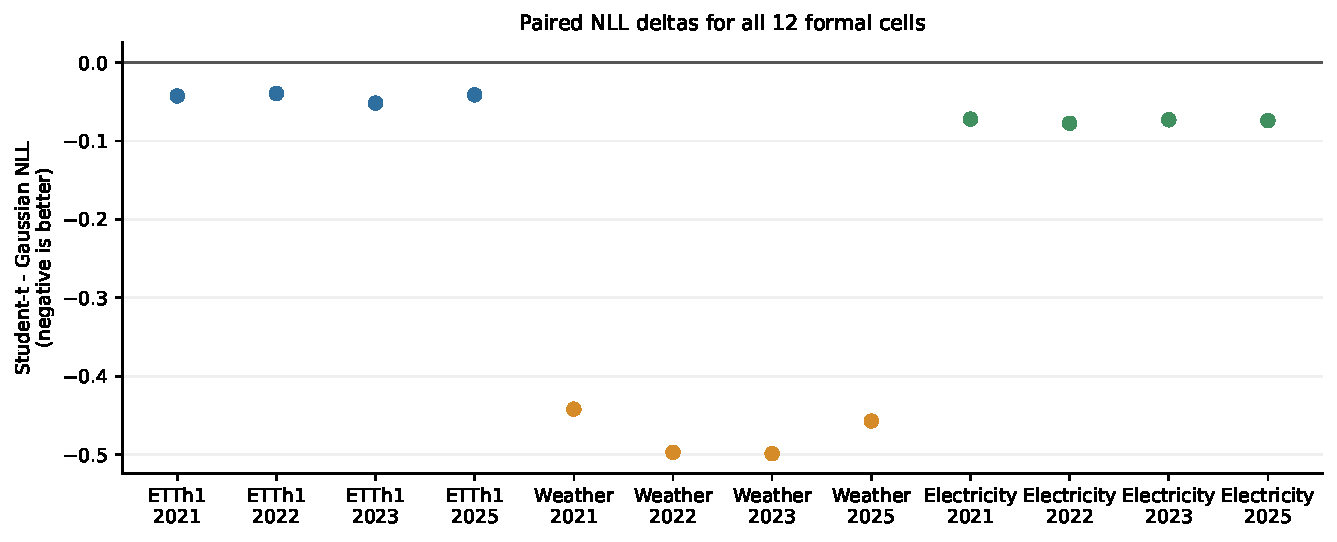
\includegraphics[width=0.96\linewidth]{fig2_multiseed_nll_deltas.pdf}
\caption{Paired TimePerceiver NLL deltas for all dataset--head-seed pairs. Negative values favor the fixed \StudentT{} forecast distribution.}
\label{fig:timeperceiver-nll}
\end{figure}

\subsection{Distribution-family ablation}
The matched-head ablation compares Gaussian, Laplace, fixed \StudentT{}, and learned-$\df$ \StudentT{} forecasts. Table~\ref{tab:distribution-ablation} and Figure~\ref{fig:distribution-ablation} support fixed heavy-tailed forecasting rather than learned degrees of freedom. Fixed $\df=8$ is sufficient under the evaluated protocol, whereas learning per-channel $\df$ provides no consistent additional benefit. The earlier learned-$\df$ results remain visible in the ablation.

\begin{table}[t]
\centering
\caption{Distribution-head ablation on frozen TimePerceiver checkpoints. Gaussian, Laplace, and fixed \StudentT{} share identical trainable location and scale capacity; lower NLL, CRPS, MSE, and MAE are better.}
\label{tab:distribution-ablation}
\scriptsize
\resizebox{\linewidth}{!}{\begin{tabular}{@{}lrrrrrr@{}}
\toprule
Dataset & Head & NLL & CRPS & MSE & Coverage error & Trainable \\
\midrule
etth1 & Gaussian & 0.918535 & 0.344127 & 0.420332 & 0.038132 & 6,168 \\
etth1 & Laplace & 0.879116 & 0.341785 & 0.424149 & 0.011910 & 6,168 \\
etth1 & Fixed Student-t (df=8) & 0.864949 & 0.336548 & 0.413927 & 0.022006 & 6,168 \\
etth1 & Learned Student-t & 0.877154 & 0.340263 & 0.419177 & 0.020301 & 6,175 \\
weather & Gaussian & 0.586325 & 0.245442 & 0.212237 & 0.082667 & 24,624 \\
weather & Laplace & 0.204399 & 0.209589 & 0.210051 & 0.070806 & 24,624 \\
weather & Fixed Student-t (df=8) & 0.136165 & 0.208461 & 0.210994 & 0.051632 & 24,624 \\
weather & Learned Student-t & 0.129293 & 0.208276 & 0.210836 & 0.052156 & 24,645 \\
electricity & Gaussian & 0.440598 & 0.209453 & 0.167881 & 0.038304 & 24,624 \\
electricity & Laplace & 0.370388 & 0.208768 & 0.170436 & 0.018222 & 24,624 \\
electricity & Fixed Student-t (df=8) & 0.367009 & 0.207797 & 0.168473 & 0.018744 & 24,624 \\
electricity & Learned Student-t & 0.366449 & 0.207786 & 0.168486 & 0.018502 & 24,945 \\
\bottomrule
\end{tabular}
}
\end{table}

\begin{figure}[t]
\centering
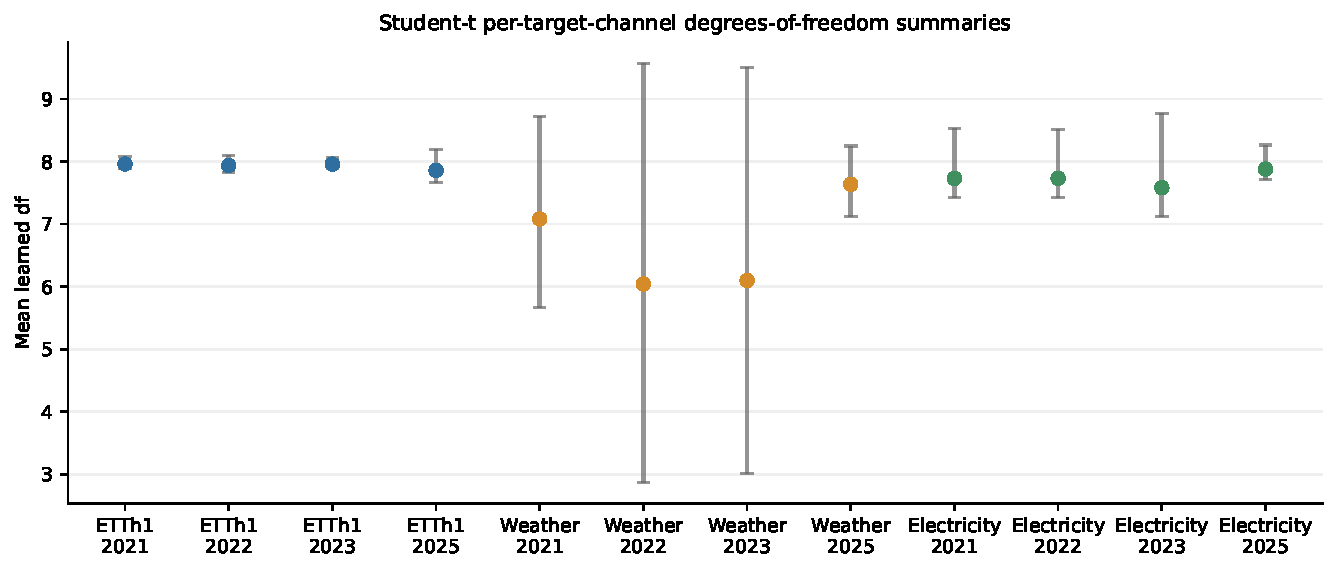
\includegraphics[width=0.88\linewidth]{fig4_student_t_df.pdf}
\caption{Distribution-head comparison under random historical missingness at rate $0.3$. The fixed $\df=8$ setting is a common reference value, not a dataset-specific selection.}
\label{fig:distribution-ablation}
\end{figure}

\subsection{PatchTST replication and point tradeoff}
PatchTST records NLL wins in 3/3 datasets, CRPS noninferiority in 3/3, point noninferiority in 2/3, and a full paired pass in 2/3. ETTh1 and Weather pass all paired criteria. For Electricity, Gaussian MSE is 0.165829 and fixed \StudentT{} MSE is 0.167809, a change of +0.001980 or +1.194\%. This exceeds the prespecified 1\% point-noninferiority threshold. Thus probabilistic-score gains transfer to the second evaluated backbone, but complete multi-metric consistency does not.

\begin{table}[t]
\centering
\caption{PatchTST fixed \StudentT{} minus Gaussian deltas. Negative NLL and CRPS values indicate improvement. Electricity's +1.194\% relative MSE change exceeds the 1\% point-noninferiority threshold.}
\label{tab:patchtst}
\scriptsize
\resizebox{\linewidth}{!}{\begin{tabular}{@{}lrrrrrrrrr@{}}
\toprule
Dataset & Backbone & $\Delta$NLL & $\Delta$CRPS & $\Delta$MSE & Rel. MSE & NLL win & CRPS NI & Point NI & Full pair \\
\midrule
ETTh1 & TimePerceiver & -0.053587 & -0.007578 & -0.006405 & -1.524\% & Yes & Yes & Yes & Yes \\
ETTh1 & PatchTST & -0.035317 & -0.002538 & -0.005439 & -1.274\% & Yes & Yes & Yes & Yes \\
Weather & TimePerceiver & -0.450160 & -0.036981 & -0.001243 & -0.586\% & Yes & Yes & Yes & Yes \\
Weather & PatchTST & -1.818698 & -0.076205 & -0.050179 & -21.595\% & Yes & Yes & Yes & Yes \\
Electricity & TimePerceiver & -0.073589 & -0.001656 & 0.000592 & +0.353\% & Yes & Yes & Yes & Yes \\
Electricity & PatchTST & -0.083433 & -0.001688 & 0.001980 & +1.194\% & Yes & Yes & No & No \\
\bottomrule
\end{tabular}
}
\end{table}

\begin{figure}[t]
\centering
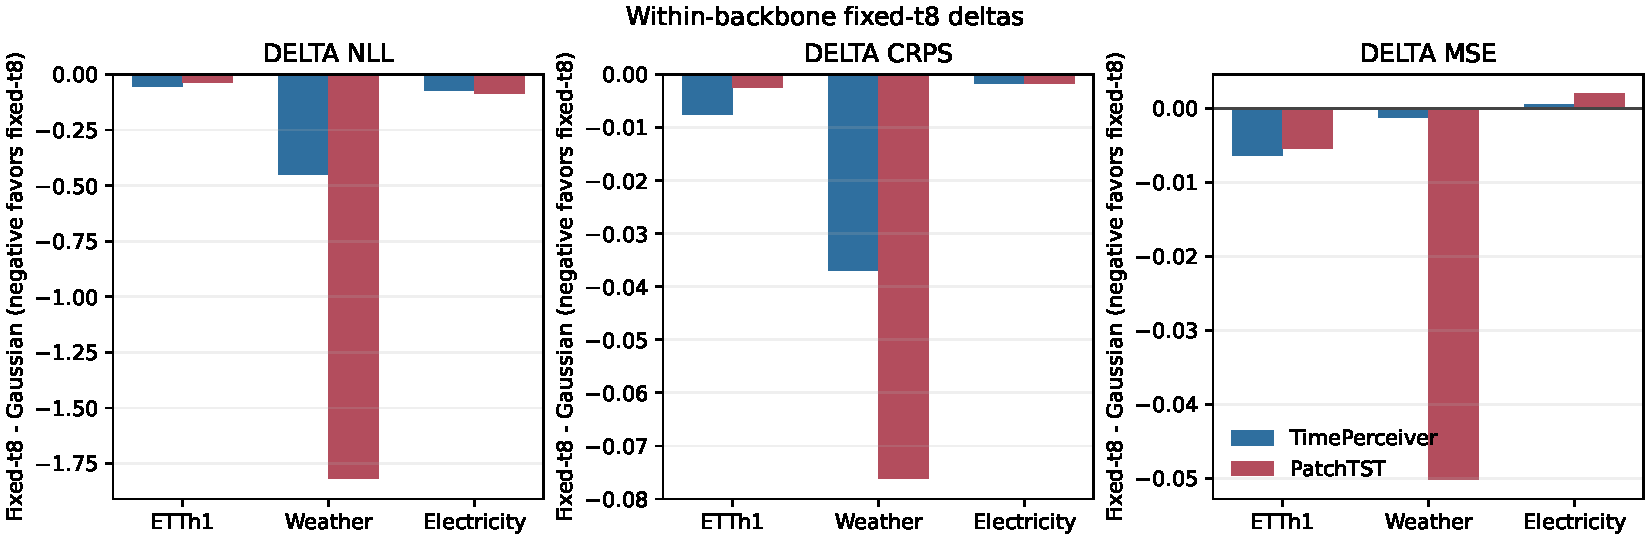
\includegraphics[width=0.96\linewidth]{fig_gate5b_cross_backbone_deltas.pdf}
\caption{Within-backbone metric deltas for TimePerceiver and PatchTST. Negative values favor fixed \StudentT{}; the positive PatchTST Electricity MSE delta is retained.}
\label{fig:cross-backbone}
\end{figure}

\subsection{Efficiency}
Fixed \StudentT{} has the same number of trainable head parameters as Gaussian and Laplace because $\df$ is not learned. Table~\ref{tab:efficiency} reports controlled timing and memory measurements. Comparisons are interpreted within each benchmark environment, not as hardware-independent throughput claims.

\begin{table}[t]
\centering
\caption{Controlled probability-head parameter, runtime, and memory measurements. Values are compared within dataset and benchmark environment.}
\label{tab:efficiency}
\scriptsize
\resizebox{\linewidth}{!}{\begin{tabular}{@{}lrrrrrr@{}}
\toprule
Dataset & Head & Params & Forward ms & NLL ms & CRPS ms & Peak MiB \\
\midrule
etth1 & Gaussian & 6,168 & 29.997997 & 51.514500 & 86.934799 & 215.033691 \\
etth1 & Laplace & 6,168 & 29.996887 & 30.016349 & 63.189127 & 215.033691 \\
etth1 & Fixed Student-t (df=8) & 6,168 & 29.902914 & 65.900001 & 90.256716 & 215.034180 \\
etth1 & Learned Student-t & 6,175 & 29.982518 & 69.371223 & 103.335362 & 215.034180 \\
weather & Gaussian & 24,624 & 59.357760 & 79.919755 & 188.685383 & 630.664551 \\
weather & Laplace & 24,624 & 58.485584 & 59.293318 & 133.341993 & 630.664551 \\
weather & Fixed Student-t (df=8) & 24,624 & 58.181018 & 98.037041 & 211.123562 & 630.665039 \\
weather & Learned Student-t & 24,645 & 59.026097 & 97.896011 & 212.516092 & 630.665039 \\
electricity & Gaussian & 24,624 & 356.894562 & 359.007118 & 1248.479182 & 4626.902832 \\
electricity & Laplace & 24,624 & 345.290164 & 343.346301 & 895.849843 & 4626.902832 \\
electricity & Fixed Student-t (df=8) & 24,624 & 343.877731 & 374.742924 & 1477.667372 & 4626.904297 \\
electricity & Learned Student-t & 24,945 & 420.384170 & 473.496327 & 1890.070674 & 4626.904297 \\
\bottomrule
\end{tabular}
}
\end{table}

\subsection{Tail-concentrated gains}
Residual-percentile decompositions place much of the NLL improvement in the most extreme Gaussian-residual bins. Figure~\ref{fig:tail-gains} presents both evaluated backbones. These diagnostics are descriptive and do not establish a causal mechanism or treat forecast elements as independent inferential samples.

\begin{figure}[t]
\centering
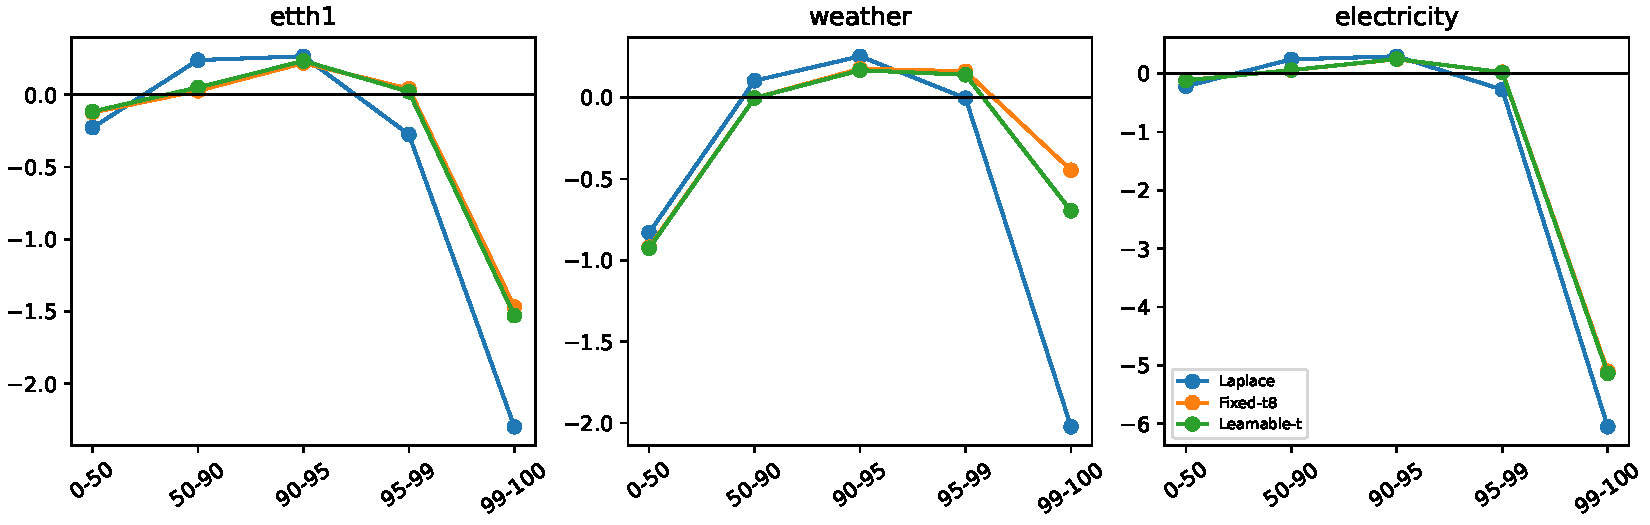
\includegraphics[width=0.48\linewidth]{fig_gate5a_tail_nll_gain.pdf}
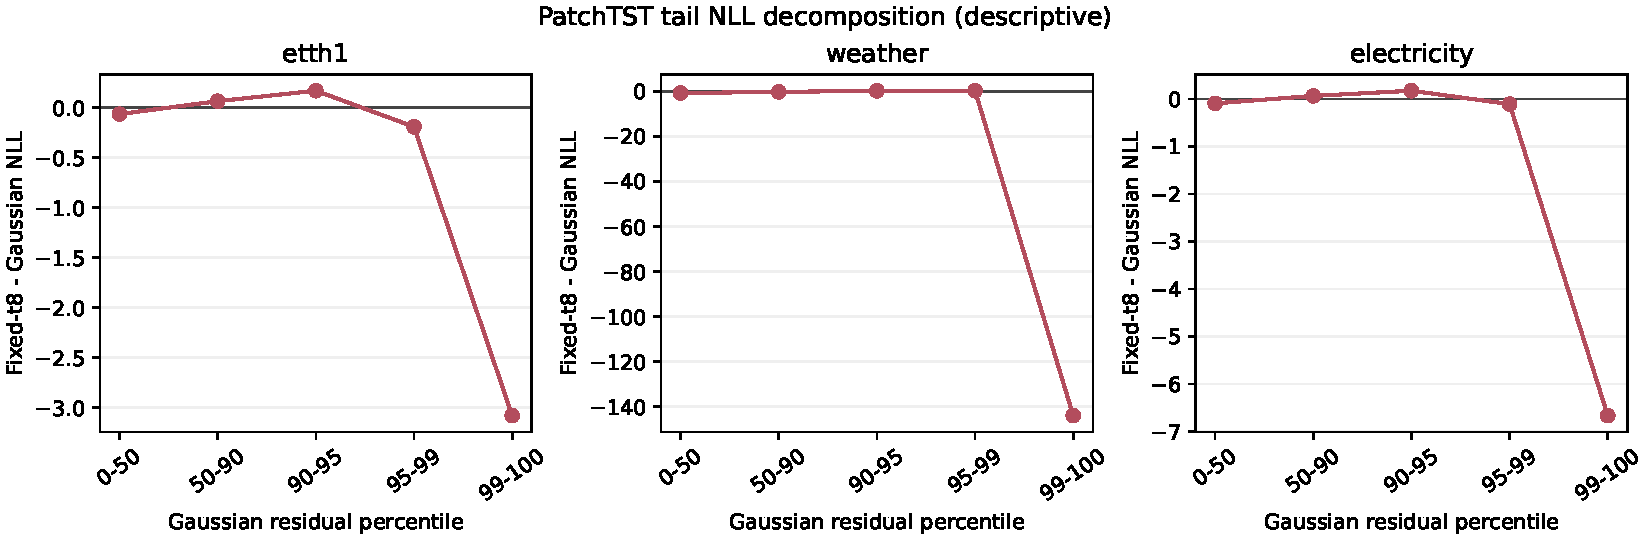
\includegraphics[width=0.48\linewidth]{fig_gate5b_patchtst_tail_nll_gain.pdf}
\caption{Descriptive NLL differences across Gaussian-residual percentile bins for TimePerceiver (left) and PatchTST (right). Negative values favor fixed \StudentT{}.}
\label{fig:tail-gains}
\end{figure}
